\section{System Overview}
The Muirkat will be deployed from the International Space Station (ISS), and as there are no onboard propulsion systems the final orbit will reflect that of the ISS. The expected orbital parameters are summarised in Figure \ref{table_orbPara}. Mission Data will be collected from multiple points throughout the orbit with the intent to develop a continuous set of data for the ioinosphere at 400km between $\pm51.6\deg latitude$.
\begin{table}[h]
	\centering
		\label{table_orbPara}
		%\begin{tabular}{ C{0.2\textwidth} p{0.8\textwidth} }
		\begin{tabular}{ lll}
				\hline
				\textbf{Parameter} & \textbf{Expected Value} &                              		
				\\ \hline
				Orbit		& %%%%%%%% add Orbit summary here		
				\\ \hline
				Perigee & 401 km & 	\multirow{5}{*}{ISS reference}\\
				Apogee & 407 km & \\
				Inclination & 51.6143 $\deg$ & \\
				Right Ascension & 333.8203 $\deg$ & \\
				Argument of Perigee & 263.8940 $\deg$ & 
			\\ \hline
			\end{tabular}
		\caption{Satellite Orbital Parameters}
	\end{table}

\begin{table}[h]
		\centering
		\label{table_ComOver}
		%\begin{tabular}{ C{0.2\textwidth} p{0.8\textwidth} }
		\begin{tabular}{ lll}
				\hline
				\textbf{Parameter} & \textbf{Expected Value} & \textbf{Description}                                		
				\\ \hline
				Communications		& %%%%%%%% add communications summary here		
				\\ \hline
				Maximum Data Link Window & 8 min & Directly passing over the ground station\\
				Average Link Time per day & 10-15min &\\
				Link time allocated per orbit  & 6 min & Based on Power Usage\\
				Minimum link time per passover & 2.5 min & For transmission of WOD and payload data 
				\\ \hline
			\end{tabular}
		\caption{Communication Overview}
	\end{table}

\begin{figure}[H]
	\centering
	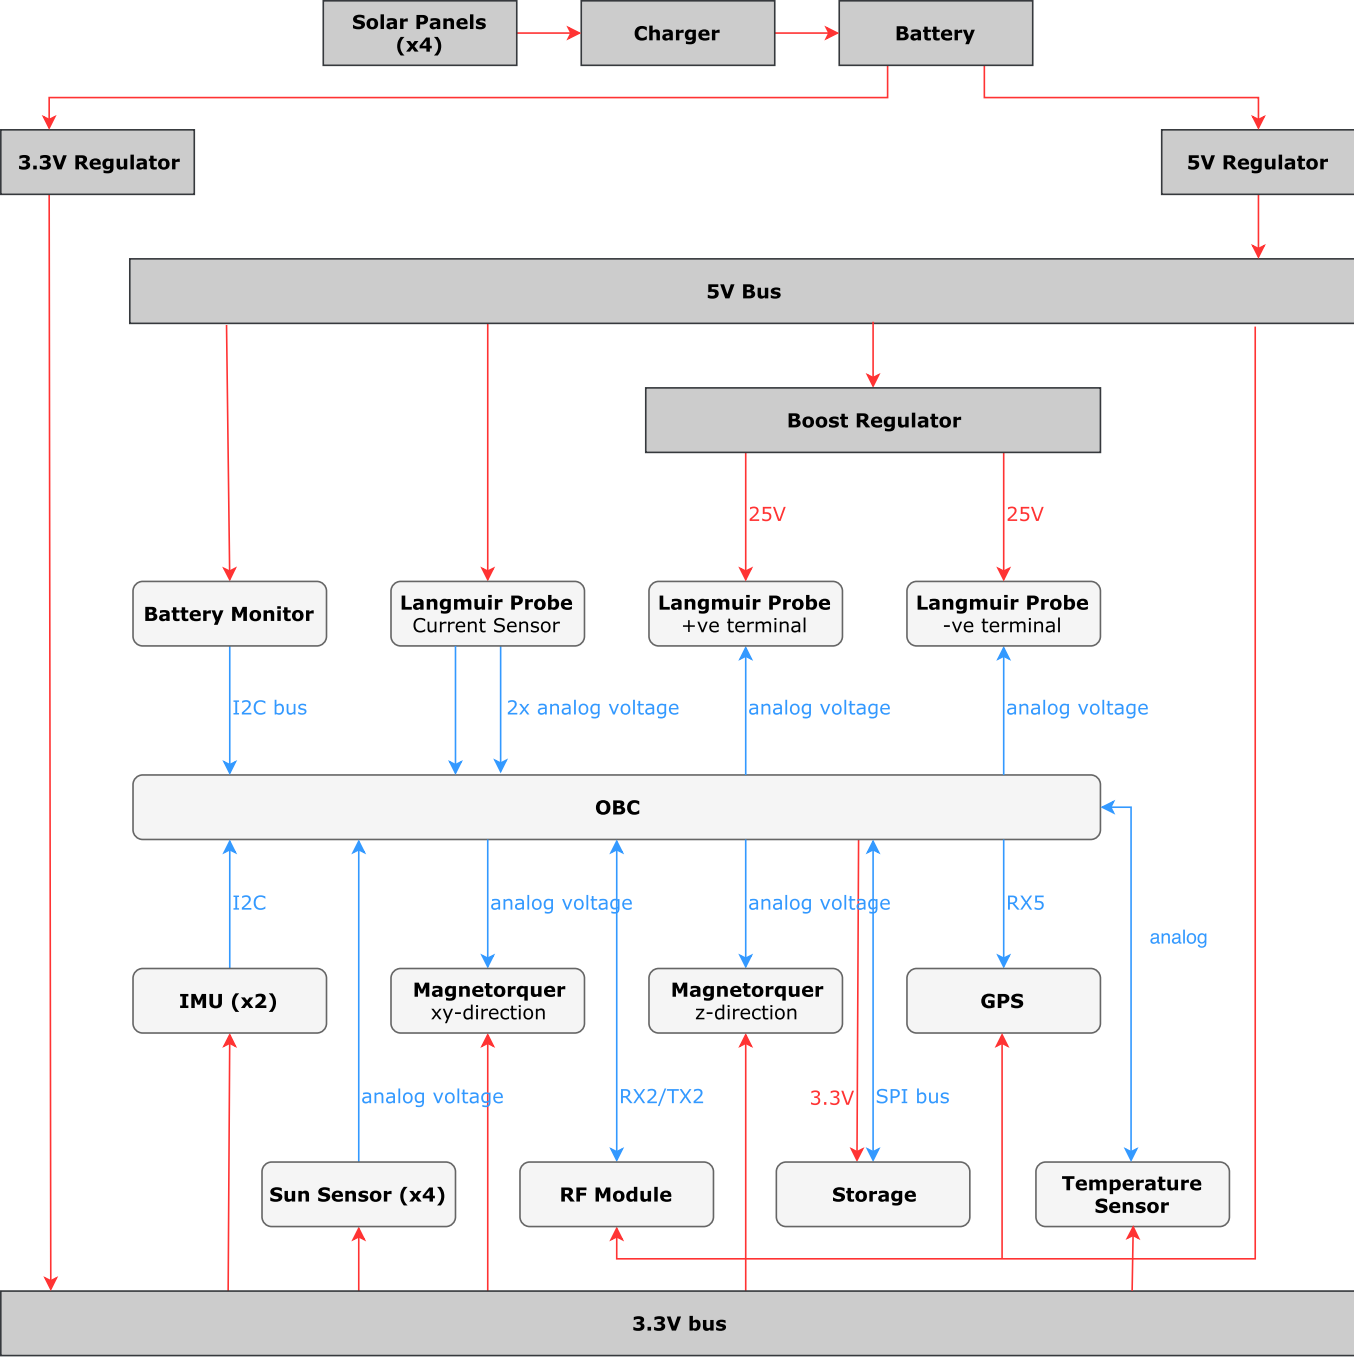
\includegraphics[scale=0.65]{flowdiag}
	\caption{Data and power flowcharts}
	\label{fig_flow}
\end{figure}
